\section{SciSpot Design}

\sysname is designed to be a cost-ware cloud resource manager for running large bags of jobs, and addresses these specific  challenges:
\begin{itemize}
\item How to 
\end{itemize}

\sysname handles all the cloud resource procurement and job scheduling associated with the bag of jobs.
Therefore, the user is only required to 







\subsection{High-level flow}

\sysname is as a cost aware cloud resource manager for running large collections of parallel jobs.
The collection forms a ``bag'' of jobs, which each job running the same executable but with different input parameters.
As explained earlier, this is a common use case.

Running a large collection of computationally similar jobs permits many cost and performance optimizations.
Given that cloud platforms offer a large number of resource configurations for their VMs, selecting the ``right'' VM for jobs can be especially beneficial in reducing the cost and running times.
Running a large number of jobs with similar computation, communication, and runtime characteristics allows us to ``explore'' the right server configuration.


The execution of a bag of job kicks off with the user providing the executable, the expected resources requirements for a single job, and the fraction of jobs that must be completed.



Therefore, \sysname's execution of a bag of jobs is composed of two serial phases.
In the first phase, we explore different cluster configurations to find the lowest cost server type.
In the second phase, we run the reminder of the jobs in the bag on the servers of the selected type (the ``exploitation'' phase).

\subsection{Server Selection for Parallel Applications}


% Maybe this can come in the earlier section?

This presents us with many challenges in the cloud-deployment of these jobs.

Cloud providers offer multiple types of instances (VMs), with different hardware configuration (such as number of CPUs and memory size).
The price of cloud servers is related to their hardware configuration, but it may not be strictly proportional to the hardware performance.
For example, a VM with 32 CPUs may not be 32 times the cost of a single CPU VM.


For parallel and distributed applications, the type of servers selected has large implications on their performance.
Consider the case of deploying an application on 8 8-core VMs vs. 16 4-core VMs.
In both cases, the total number of CPU cores is the same.
However, the larger number of VMs requires more communication between the application tasks, and thus may result in performance degradation.
The performance of applications at different cluster configurations depends on their communication patterns and scaling properties. 



Thus, when deploying applications on the cloud, one has to mindful of the cost and performance tradeoff.
However, in the case of transient servers, the story does not stop here. 


In addition to pricing differences, the transient availability of instances \emph{also} differs by type.
Because the availability of a transient VM is broadly determined by the overall supply and demand of the instances of that \emph{particular} type, the ``preemption rate'' of VMs often depends on the type of the instance.



Thus, selecting a transient cloud server involves a complex tradeoff between the cost of servers, their performance, and the preemption-rate.
We develop server selection policies in the next section.


\begin{figure}
  \centering 
  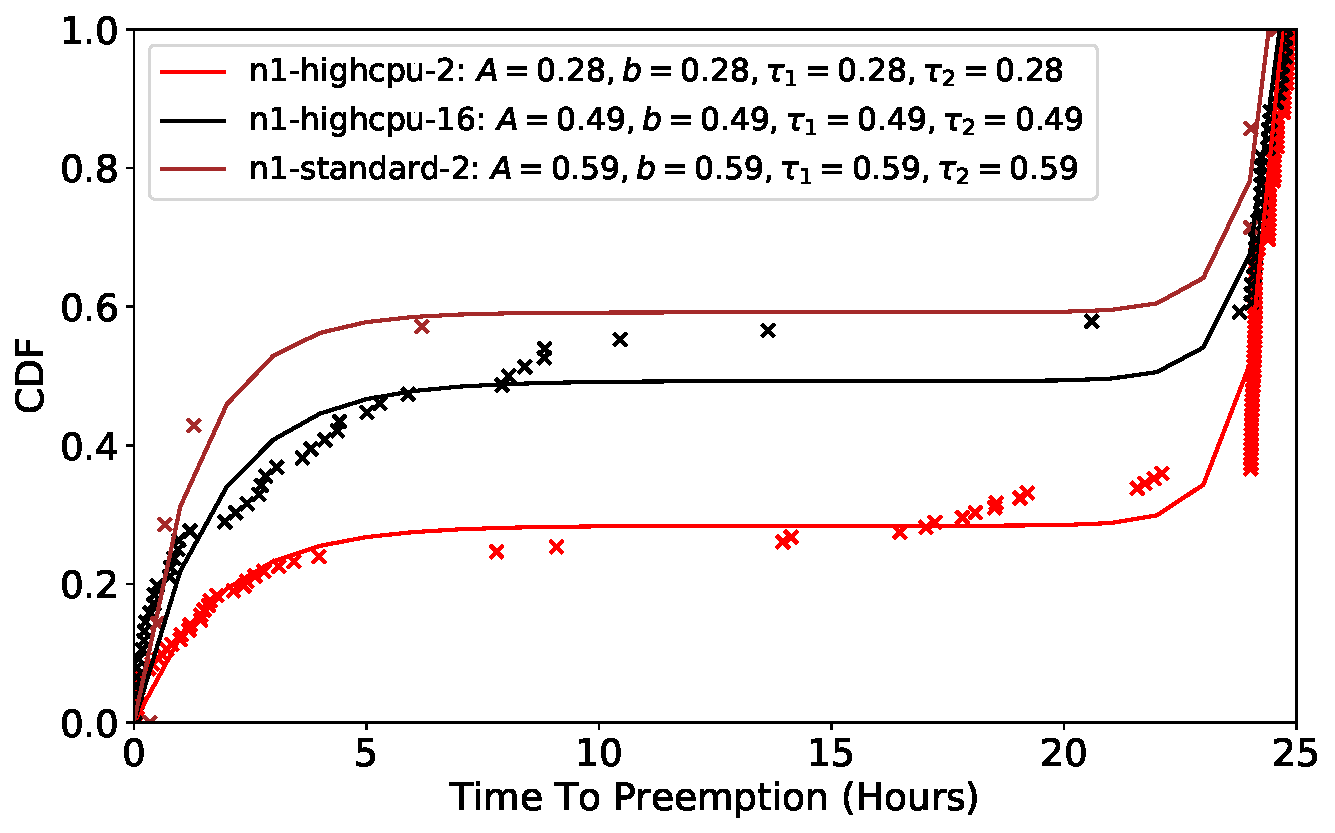
\includegraphics[width=0.4\textwidth]{../graphs/cdf_comparison_3.pdf}
  \caption{The preemption characteristics of different VM types. Larger VMs are more likely to be preempted}
  \label{fig:cdf-comparison}
\end{figure}

\sysname's server selection policy seeks to identify the best server type for a given job-group.

As stated in the previous subsection, the transient server selection problem is challenging because it involves balancing multiple optimization criteria: applications want low cost, low preemptions, and high performance.

Server selection based on application characteristics is a subject of a growing amount of recent work.
These approaches often use micro benchmarks to gather performance data of cloud servers, and then use application performance models to determine suitable VMs for a specific application.
Another class of approaches uses ``black box'' performance modeling, where the application's performance is modeled using a function of the resources, for example, by using linear regression.

In contrast to prior work, our server selection employs a ``cold start'' policy, and we do not run profiling or pilot jobs that can increase the overall running time and cost.
Instead, we search for the ``best'' cluster configuration for jobs in a job-group, by exploring the cluster configuration space for the ``optimum'' server type that optimizes all the desired parameters: cost, running time, and revocation rate.


Thus, the first $e$ jobs in the job group $J_1\ldots J_e$ are the exploration jobs, run on different cluster configurations.
We limit the total number of combinations to explore, by allowing users to submit an estimate of the total number of CPU cores that they desire for each job.
This allows us to meet the user expectations in terms of performance and cost---whether the user expects us to spend a large amount of resources or not.

Thus, assuming that there are $s$ different types of VM instances, the first $s$ jobs are run on the $s$ different types.
Note that we use homogeneous clusters, since the performance of BSP programs in Heterogeneous environments can be degraded, and importantly, as we show, there are no performance or cost benefits to Heterogenity. 


For each server type $i$, we calcuate the expected cost $E[C_i]$.

$E[C_i] = n_i*c_i * E[T_i]$, where $c_i$ is the price (per second) of the server, $n_i$ is the number of servers of that type required to meet the core-count requirement.
The expected running time of the job depends on two factors: the actual running time $T$, and the increase in running time due to preemptions.
Each preemption is akin to a fail-stop failure, which requires an application to restart.
Our system makes no assumptions about the fault-tolerance policies supported by the application. For example, some applications may be able to \emph{checkpoint} their state periodically.
In either case (checkpointing or not), there is some work lost due to revocations.
For ease of exposition, we assume no checkpointing. We discuss checkpointing in the next section (or never?)


\mhead{Expected running time:}
Let the running time without failure be T:

\begin{equation}
  \label{eq:et1}
E[T_i] = T + P(\text{at least one failure})*T/2   
\end{equation}

For calcuating the probability of failure, we assume that the failure rate of an individual server of the type is $p_i$. 

\begin{align}
  \label{eq:pfail1}
  P(\text{at least one failure}) &= 1-P(\text{no failure}) \\
                                 &= 1-(1-p_i)^{n_i} 
\end{align}

Thus, we can see that if we select smaller VMs, we will require more of them (higher $n_i$), and this cluster configuration will have a larger probability of failure and thus higher running times and costs.

The probability of failure $p_i$ depends on the type of server, and we use historically determined failure distributions.
Roughly, if we assume exponentially distributed failures, then:
\begin{equation}
  \label{eq:pi}
  p_i = \dfrac{T}{\text{MTTF}_i}
\end{equation}

Where MTTF is the mean time to failure of the server type, and T is the empirically determined job running time without failures (the best case).





In addition to searching over the servers, the effective number of servers is also dynamic in the case of transient environments due to preemptions.
Thus, once we have found the appropriate server, we then explore the application's performance at smaller cluster sizes, which helps in the job-group policies that we discuss next. 

\subsection{Scheduling a Bag of Jobs}

How jobs are generated

\textbf{Generating Jobs For a Bag:} Optionally, \sysname can also take as input a description of the (multi-dimensional) parameter space, and then generate the jobs.
We do this with the users specifying the values that different job parameters can take, and then producing a list with all the permutations.
Because job-failures can cause some parameter combinations to remain unexplored, we strive for uniformity of sampling by randomizing the order in which jobs in a bag are scheduled, so that we don't end up in a situation with a large fraction of any parameter remaining unexplored if the completion threshold has been met.


More details are provided in the Interface and Implementation section.


How jobs are scheduled.

How many jobs to run in parallel (deadline and exploration sweep based)

What to do on failure


%\subsection{Preemption-handling Policies}

We run the remaining jobs on the right configuration that is determined through the server selection policy.

Our goal is to minimize costs given a deadline.

This determines two things: how many jobs should be run in parallel, and what to do upon a revocation.

The number of jobs in parallel determines the overall size of our cluster.

$\text{number of parallel jobs} = \dfrac{N\cdot T}{\text{Deadline Duration}}$

If a server is preempted, then the job running on it will cease to run.
Our preemption handling policies then decide what to do:
\begin{enumerate}
\item Restart the job on a smaller number of servers 
\item Replenish lost servers and restart job
\item Discard job. This may be useful in case of parameter sweeps. 
\end{enumerate}

In addition, the user is also allowed to provide the fraction of jobs that are allowed to fail ($\eta$).

We exploit the naturally occuring intra-job redundancy. 

\mhead{New jobs.}
For new jobs, the questions are similar to the preemption policy ones, because they also must take into account the failures.

That is, assume that a job has finished and it is time to run a new job. So now, we have a set of servers that successfully ran a job. If we run on same set, then we may hit the 24 hour wall. But, if we discard these and launch new ones, then we face the infant mortality problem. So the question is, at what age should servers be retired? If they are too close to EOL (24 hours), then what's the point? Better start something fresh.



% \subsection{Checkpointing}

% Checkpointing requires the same number of servers, which may be tricky, whereas restarts can be on smaller number of nodes no problem.

% Maybe talk about the dynamic programming based checkpointing here?



% \subsection{Early Stopping}

% Based on the energy function, we can stop some simulations early.
% The early stopping criteria helps in minimizing the number of jobs run to completion.

% We use this to proactively monitor jobs, as well as to decide whether to restart a job if it is preempted.

% *This can be a fairly substantial section*



\begin{comment}
Scientific simulation applications consume a large amount of computational resources, and are often used in the context of \emph{exploratory} research, where a large amount of jobs are run with  different simulation parameters.
This can be either a \emph{parameter sweep}, where a large number of parameters need to be evaluated, or a \emph{search} over a large parameter space for the ``right'' set of parameters that yield the desired model behavior.

In this paper, we look at the problem of running scientific simulations on \emph{transient} computing resources in public clouds. 


Past work has largely been focused on running parallel jobs (such as MPI) in the cloud. 
However, considering entire \emph{job-groups} or ensembles of jobs presents new challenges and opportunities in timely, low-cost computation.

Our system, \sysname, is a unified framework for running large job-groups that result from parameter exploration. 

Input and some assumptions:
We assume that the job-group consists of $J_1\ldots J_N$, with each job evaluating a model on some parameter.
The list of parameters to explore can either be generated apriori (as in the case of parameter sweeps), or be dynamically generated as in the case of a search.

In this section, we will look at how we address these challenges:
\begin{enumerate}
\item How to select the right type of cloud server for an application?
\item How to effectively run job-groups?
\end{enumerate}



Job-groups are executed in two phases.
In the first phase, we search for the right type of server for the jobs in the job-group, and then in the second phase, we execute the remaining jobs on the chosen servers.
\end{comment}



%%% Local Variables:
%%% mode: latex
%%% TeX-master: "paper"
%%% End:
